\documentclass[a4paper,11pt,fleqn,twoside,openright]{memoir} 	% Openright aabner kapitler paa hoejresider (openany begge)

%%%% PACKAGES %%%%

% ¤¤ Oversaettelse og tegnsaetning ¤¤ %
%tilføjet af AT
\usepackage{url}
\usepackage{rotating}
\usepackage{pdflscape}

\usepackage[utf8]{inputenc}					% Input-indkodning af tegnsaet (UTF8)
\usepackage[danish]{babel}					% Dokumentets sprog
\usepackage[T1]{fontenc}					% Output-indkodning af tegnsaet (T1)
\usepackage{ragged2e,anyfontsize}			% Justering af elementer
\usepackage{fixltx2e}						% Retter forskellige fejl i LaTeX-kernen	
								\usepackage{blindtext}	
								
% ¤¤ Figurer og tabeller (floats) ¤¤ %
\usepackage{graphicx} 						% Haandtering af eksterne billeder (JPG, PNG, PDF)
\usepackage{multirow}                		% Fletning af raekker og kolonner (\multicolumn og \multirow)
\usepackage{colortbl} 						% Farver i tabeller (fx \columncolor, \rowcolor og \cellcolor)
\usepackage[dvipsnames]{xcolor}				% Definer farver med \definecolor. Se mere: http://en.wikibooks.org/wiki/LaTeX/Colors
\usepackage{flafter}						% Soerger for at floats ikke optraeder i teksten foer deres reference
\let\newfloat\relax 						% Justering mellem float-pakken og memoir
\usepackage{float}							% Muliggoer eksakt placering af floats, f.eks. \begin{figure}[H]
%\usepackage{eso-pic}						% Tilfoej billedekommandoer paa hver side
%\usepackage{wrapfig}						% Indsaettelse af figurer omsvoebt af tekst. \begin{wrapfigure}{Placering}{Stoerrelse}
%\usepackage{multicol}         	        	% Muliggoer tekst i spalter
%\usepackage{rotating}						% Rotation af tekst med \begin{sideways}...\end{sideways}
\usepackage{longtable}

% ¤¤ Matematik mm. ¤¤
\usepackage{amsmath,amssymb,stmaryrd} 		% Avancerede matematik-udvidelser
\usepackage{mathtools}						% Andre matematik- og tegnudvidelser
\usepackage{textcomp}                 		% Symbol-udvidelser (f.eks. promille-tegn med \textperthousand )
\usepackage{siunitx}						% Flot og konsistent praesentation af tal og enheder med \si{enhed} og \SI{tal}{enhed}
\sisetup{output-decimal-marker = {,}}		% Opsaetning af \SI (DE for komma som decimalseparator) 
\usepackage[version=3]{mhchem} 				% Kemi-pakke til flot og let notation af formler, f.eks. \ce{Fe2O3}
%\usepackage{rsphrase}						% Kemi-pakke til RS-saetninger, f.eks. \rsphrase{R1}

% ¤¤ Referencer og kilder ¤¤ %
\usepackage[danish]{varioref}				% Muliggoer bl.a. krydshenvisninger med sidetal (\vref)
\usepackage{natbib}							% Udvidelse med naturvidenskabelige citationsmodeller
%\usepackage{xr}							% Referencer til eksternt dokument med \externaldocument{<NAVN>}
%\usepackage{glossaries}					% Terminologi- eller symbolliste (se mere i Daleifs Latex-bog)

% ¤¤ Misc. ¤¤ %
\usepackage{listings}						% Placer kildekode i dokumentet med \begin{lstlisting}...\end{lstlisting}
\usepackage{lipsum}							% Dummy text \lipsum[..]
\usepackage[shortlabels]{enumitem}			% Muliggoer enkelt konfiguration af lister
\usepackage{pdfpages}						% Goer det muligt at inkludere pdf-dokumenter med kommandoen \includepdf[pages={x-y}]{fil.pdf}	
\pdfoptionpdfminorversion=6					% Muliggoer inkludering af pdf dokumenter, af version 1.6 og hoejere
\pretolerance=2500 							% Justering af afstand mellem ord (hoejt tal, mindre orddeling og mere luft mellem ord)

% Kommentarer og rettelser med \fxnote. Med 'final' i stedet for 'draft' udloeser hver note en error i den faerdige rapport.
\usepackage[footnote,draft,danish,silent,nomargin]{fixme}		


%%%% CUSTOM SETTINGS %%%%

% ¤¤ Marginer ¤¤ %
\setlrmarginsandblock{3.5cm}{2.5cm}{*}		% \setlrmarginsandblock{Indbinding}{Kant}{Ratio}
\setulmarginsandblock{2.5cm}{3.0cm}{*}		% \setulmarginsandblock{Top}{Bund}{Ratio}
\checkandfixthelayout 						% Oversaetter vaerdier til brug for andre pakker

%	¤¤ Afsnitsformatering ¤¤ %
\setlength{\parindent}{0mm}           		% Stoerrelse af indryk
\setlength{\parskip}{3mm}          			% Afstand mellem afsnit ved brug af double Enter
\linespread{1,1}							% Linie afstand

% ¤¤ Litteraturlisten ¤¤ %
\bibpunct[,]{[}{]}{;}{a}{,}{,} 				% Definerer de 6 parametre ved Harvard henvisning (bl.a. parantestype og seperatortegn)
\bibliographystyle{bibtex/harvard}			% Udseende af litteraturlisten.

% ¤¤ Indholdsfortegnelse ¤¤ %
\setcounter{secnumdepth}{4}		 			% Dybden af nummerede overkrifter (part/chapter/section/subsection)
\setcounter{maxsecnumdepth}{4}					% Dokumentklassens graense for nummereringsdybde
\setcounter{tocdepth}{4} 					% Dybden af indholdsfortegnelsen

% ¤¤ Lister ¤¤ %
\setlist{
  topsep=0pt,								% Vertikal afstand mellem tekst og listen
  itemsep=-1ex,								% Vertikal afstand mellem items
} 

% ¤¤ Visuelle referencer ¤¤ %
\usepackage[colorlinks]{hyperref}			% Danner klikbare referencer (hyperlinks) i dokumentet.
\hypersetup{colorlinks = true,				% Opsaetning af farvede hyperlinks (interne links, citeringer og URL)
    linkcolor = black,
    citecolor = black,
    urlcolor = black
}

% ¤¤ Opsaetning af figur- og tabeltekst ¤¤ %
\captionnamefont{\small\bfseries\itshape}	% Opsaetning af tekstdelen ('Figur' eller 'Tabel')
\captiontitlefont{\small}					% Opsaetning af nummerering
\captiondelim{. }							% Seperator mellem nummerering og figurtekst
\hangcaption								% Venstrejusterer flere-liniers figurtekst under hinanden
\captionwidth{\linewidth}					% Bredden af figurteksten
\setlength{\belowcaptionskip}{0pt}			% Afstand under figurteksten
		
% ¤¤ Opsaetning af listings ¤¤ %
\definecolor{commentGreen}{RGB}{34,139,24}
\definecolor{stringPurple}{RGB}{208,76,239}

\lstset{language=Matlab,					% Sprog
	basicstyle=\ttfamily\scriptsize,		% Opsaetning af teksten
	keywords={for,if,while,else,elseif,		% Noegleord at fremhaeve
			  end,break,return,case,
			  switch,function},
	keywordstyle=\color{blue},				% Opsaetning af noegleord
	commentstyle=\color{commentGreen},		% Opsaetning af kommentarer
	stringstyle=\color{stringPurple},		% Opsaetning af strenge
	showstringspaces=false,					% Mellemrum i strenge enten vist eller blanke
	numbers=left, numberstyle=\tiny,		% Linjenumre
	extendedchars=true, 					% Tillader specielle karakterer
	columns=flexible,						% Kolonnejustering
	breaklines, breakatwhitespace=true,		% Bryd lange linjer
}

% ¤¤ Navngivning ¤¤ %
\addto\captionsdanish{
	\renewcommand\appendixname{Appendiks}
	\renewcommand\contentsname{Indholdsfortegnelse}	
	\renewcommand\appendixpagename{Appendiks}
	\renewcommand\appendixtocname{Appendiks}
	\renewcommand\cftchaptername{\chaptername~}				% Skriver "Kapitel" foran kapitlerne i indholdsfortegnelsen
	\renewcommand\cftappendixname{\appendixname~}			% Skriver "Appendiks" foran appendiks i indholdsfortegnelsen
}

% ¤¤ Kapiteludssende ¤¤ %
\definecolor{numbercolor}{gray}{0.7}		% Definerer en farve til brug til kapiteludseende
\newif\ifchapternonum

\makechapterstyle{jenor}{					% Definerer kapiteludseende frem til ...
  \renewcommand\beforechapskip{0pt}
  \renewcommand\printchaptername{}
  \renewcommand\printchapternum{}
  \renewcommand\printchapternonum{\chapternonumtrue}
  \renewcommand\chaptitlefont{\fontfamily{pbk}\fontseries{db}\fontshape{n}\fontsize{25}{35}\selectfont\raggedleft}
  \renewcommand\chapnumfont{\fontfamily{pbk}\fontseries{m}\fontshape{n}\fontsize{1in}{0in}\selectfont\color{numbercolor}}
  \renewcommand\printchaptertitle[1]{%
    \noindent
    \ifchapternonum
    \begin{tabularx}{\textwidth}{X}
    {\let\\\newline\chaptitlefont ##1\par} 
    \end{tabularx}
    \par\vskip-2.5mm\hrule
    \else
    \begin{tabularx}{\textwidth}{Xl}
    {\parbox[b]{\linewidth}{\chaptitlefont ##1}} & \raisebox{-15pt}{\chapnumfont \thechapter}
    \end{tabularx}
    \par\vskip2mm\hrule
    \fi
  }
}											% ... her

\chapterstyle{jenor}						% Valg af kapiteludseende - Google 'memoir chapter styles' for alternativer

% ¤¤ Sidehoved ¤¤ %

\makepagestyle{Uni}							% Definerer sidehoved og sidefod udseende frem til ...
\makepsmarks{Uni}{%
	\createmark{chapter}{left}{shownumber}{}{. \ }
	\createmark{section}{right}{shownumber}{}{. \ }
	\createplainmark{toc}{both}{\contentsname}
	\createplainmark{lof}{both}{\listfigurename}
	\createplainmark{lot}{both}{\listtablename}
	\createplainmark{bib}{both}{\bibname}
	\createplainmark{index}{both}{\indexname}
	\createplainmark{glossary}{both}{\glossaryname}
}
\nouppercaseheads											% Ingen Caps oenskes

\makeevenhead{Uni}{Langerhanske Øer}{}{\leftmark}				% Definerer lige siders sidehoved (\makeevenhead{Navn}{Venstre}{Center}{Hoejre})
\makeoddhead{Uni}{\rightmark}{}{Ingeniørhøjskolen Aarhus}			% Definerer ulige siders sidehoved (\makeoddhead{Navn}{Venstre}{Center}{Hoejre})
\makeevenfoot{Uni}{\thepage}{}{}							% Definerer lige siders sidefod (\makeevenfoot{Navn}{Venstre}{Center}{Hoejre})
\makeoddfoot{Uni}{}{}{\thepage}								% Definerer ulige siders sidefod (\makeoddfoot{Navn}{Venstre}{Center}{Hoejre})
\makeheadrule{Uni}{\textwidth}{0.5pt}						% Tilfoejer en streg under sidehovedets indhold
\makefootrule{Uni}{\textwidth}{0.5pt}{1mm}					% Tilfoejer en streg under sidefodens indhold

\copypagestyle{Unichap}{Uni}								% Sidehoved for kapitelsider defineres som standardsider, men med blank sidehoved
\makeoddhead{Unichap}{}{}{}
\makeevenhead{Unichap}{}{}{}
\makeheadrule{Unichap}{\textwidth}{0pt}
\aliaspagestyle{chapter}{Unichap}							% Den ny style vaelges til at gaelde for chapters
															% ... her
															
\pagestyle{Uni}												% Valg af sidehoved og sidefod (benyt "plain" for ingen sidehoved/fod)


%%%% CUSTOM COMMANDS %%%%

% ¤¤ Billede hack ¤¤ %										% Indsaet figurer nemt med \figur{Stoerrelse}{Fil}{Figurtekst}{Label}
\newcommand{\figur}[4]{
		\begin{figure}[H] \centering
			\includegraphics[width=#1\textwidth]{billeder/#2}
			\caption{#3}\label{#4}
		\end{figure} 
}

% ¤¤ Specielle tegn ¤¤ %
\newcommand{\decC}{^{\circ}\text{C}}
\newcommand{\dec}{^{\circ}}
\newcommand{\m}{\cdot}


%%%% ORDDELING %%%%

\hyphenation{}											% Preamble indlaeses
\raggedbottom													% Soerger for at LaTeX ikke "straekker" teksten

%\includeonly{file1,file2}										% Inkluder kun specifikke filer (kommasepareret liste)

\begin{document}												% Starter dokumentet - obligatorisk


\frontmatter													% Forindhold - nummereres med romertal

\thispagestyle{empty}
\begin{center}
\vspace{3cm}

\phantom{hul}

\phantom{hul}

\phantom{hul}

\textsl{\LARGE Cell sorter for isolation of insulin producing cells} \\ \vspace{0.25cm}
\textsl{\Large Projektdokumentation} \\ %\vspace{1cm}

\rule{13cm}{3mm} \\ \vspace{1cm}

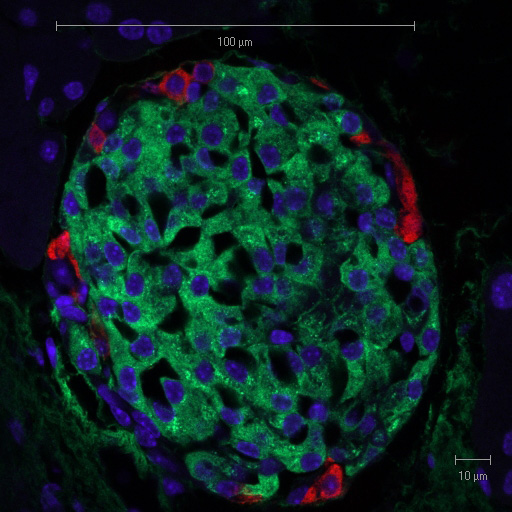
\includegraphics[width=0.9\textwidth]{billeder/forside.jpg}

\textsc{\center Bachelorprojekt \\
Projektnr: 15137 \\
Ingeniørhøjskolen, Aarhus Universitet \\
Den 16. december 2015 \\ \vspace{1cm}
11242	Anders Toft Andersen \\
201270874	Anders Esager \\
Projektvejleder: Samuel Alberg Thrysøe \\}
\end{center}

\cleardoublepage												% Indsaetter tom side, saa naeste kapitel starter paa hoejre side (hvis noedvendigt)
%% Dette er et titelblad designet til videregående uddannelser på et universitet
% Filen kræver:
% Universitetets logo:  AU-logo-DK eller AU-logo-DK
% Synopsis: En fil ved navn synopsis.tex

% Udarbejdet af: Jesper Nørgaard (jesper@noergaard.eu) 10. april 2012

\phantomsection
\pdfbookmark[0]{Titelblad}{titelblad}
\thispagestyle{empty}

\begin{minipage}[t]{0.48\textwidth}
\vspace*{-8pt}			

\includegraphics[height=2.5cm]{billeder/AU-logo-DK}
\end{minipage}
\hfill
\begin{minipage}[t]{0.48\textwidth}
{\small 
\textbf{Studienævn for Aarhus School of Science}\\
Nordre Ringgade 1 \\
8000 Aarhus C \\
Tlf: 8715 0000 \\
http://www.au.dk}
\end{minipage}

\vspace*{1cm}

\begin{minipage}[t]{0.48\textwidth}
\textbf{Titel:} \\[5pt]\bigskip\hspace{2ex}
Energirenovering

\textbf{Projekt:} \\[5pt]\bigskip\hspace{2ex}
P1-projekt

\textbf{Projektperiode:} \\[5pt]\bigskip\hspace{2ex}
September 2014 - December 2014

\textbf{Projektgruppe:} \\[5pt]\bigskip\hspace{2ex}
B131	

\textbf{Deltagere:} \\[5pt]\hspace*{2ex}
Adam  G. Hansen \\\hspace*{2ex}
Berit Jørgensen \\\hspace*{2ex}
Christoffer Haning \\\hspace*{2ex}
Dorthe Møller \\\hspace*{2ex}
Ejnar V. Jensen \\\hspace*{2ex}
Freja Poulsen \\\bigskip\hspace{2ex}
Gerhard Pedersen

\textbf{Vejledere:} \\[5pt]\hspace*{2ex}
Carsten Henningsen \\\bigskip\hspace{2ex}
Lotte Dalgaard

\vspace*{1cm}

\textbf{Oplagstal: 10} \\
\textbf{Sidetal: 80} \\
\textbf{Appendiks: 3} \\ 
\textbf{Afsluttet 18-12-2014}

\end{minipage}
\hfill
\begin{minipage}[t]{0.483\textwidth}
Synopsis: \\[5pt]
\fbox{\parbox{7cm}{\bigskipSynopsis

\bigskip}}
\end{minipage}

\vfill

{\footnotesize\itshape Rapportens indhold er frit tilgængeligt, men offentliggørelse (med kildeangivelse) må kun ske efter aftale med forfatterne.}

% Rapportens indhold er frit tilgængeligt, men offentliggørelse (med kildeangivelse) må kun ske efter aftale med forfatterne.
% The content of the report is freely available, but publication (with source reference) may only take place in agreement with the authors.

%\cleardoublepage
\chapter*{Forord}

Denne rapport er udarbejdet som en del af syvende semesters bachelorprojekt på Ingeniørhøjskolen, Aarhus Universitet. Rapporten er udarbejdet af en projektgruppe bestående af 2 sundhedsteknologistuderende. Projektet er udarbejdet i samarbejde med Søren Gregersen, overlæge på Medicinsk Endokrinologisk Afdeling på Aarhus Universitetshospital med hjælp fra Per. B. Jeppesen, Lektor ved Institut for Klinisk Medicin, Aarhus Universitet. Bachelorprojektet er udført i perioden 28. august 2015 til 16. december 2015, hvor forprojektet er udført i perioden 26. april 2015 til 15. juni 2015.  

Projektgruppen retter en stor tak til Søren Gregersen for samarbejdet, ligeledes skal der gives en tak til Per B. Jeppesen. Ydermere skal der lyde en varm tak til gruppens vejleder Samuel Thrysøe, der har hjulpet og støttet gruppen igennem hele processen. Endelig skal der gives en tak til reviewgruppen bestående af Simon Vammen Grønbæk og Karl-John Schmidt, som har bestået med konstruktiv kritik og rettelser. 


%Dette dokument indeholder projektdokumentationen for projektet \textit{Cell sorter for isolation of insulin producing cells}. Dokumentet indeholder kravspecifikation og accepttest for systemet, samt beskrivelse af projektets design og implementeringsfase. 

%Kravspecifikationen er udarbejdet i samarbejde med Søren Gregersen, overlæge på Medicinsk Endokrinologisk Afdeling, Aarhus Universitetshospital, der agerer som projektets kunde. 



\phantom{Luft}

\phantom{Luft}

\begin{table}[H]
	\centering
		\begin{tabular}{c c}
			\underline{\phantom{mmmmmmmmmmmmmm}} & \underline{\phantom{mmmmmmmmmmmmmm}}  \\
			Anders Toft Andersen			& Anders Esager		 			\\ 										\end{tabular}
\end{table}

\section*{Læsevejledning}
Rapporten indeholder primært metoder, resultater og diskussioner til produktet, som gruppen har udarbejdet. Der vil igennem rapporten fremtræde kildehenvisninger, og disse vil være samlet i en kildeliste bagerst i rapporten. Der er i rapporten anvendt kildehenvisning efter Harvardmetoden, i teksten refereres en kilde med [Efternavn, År]. Denne henvisning fører til kildelisten, hvor bøger er angivet med forfatter, titel, udgave og forlag, mens internetsider er angivet med forfatter, titel og dato. Til sidst i rapporten er bilagsliste, som anskueliggør filnavnene i den afleverede bilagsmappen. Diagrammerne udarbejdet i projektet er skrevet på engelsk. 

I bilagslisten forefindes alle filerne, der er afleveret ved siden af rapporten, herunder datablade, Matlab-kode, Eagle kilde-filer og Gerber-filer. Herudover er den udfyldte accepttest og fejlrapport vedlagt som bilag.

Ved siden af rapporten er vedlagt en video, som viser den udviklede prototype.

%Der vil igennem rapporten fremtræde kildehenvisninger, og disse vil være samlet i en kildeliste bagerst i rapporten. Der er i rapporten anvendt kildehenvisning efter Harvardmetoden, så i teksten refereres en kilde med [Efternavn, År]. Denne henvisning fører til kildelisten, hvor bøger er angivet med forfatter, titel, udgave og forlag, mens Internetsider er angivet med forfatter, titel og dato. Figurer og tabeller er nummereret i henhold til kapitel, dvs. den første figur i kapitel 7 har nummer 7.1, den anden, nummer 7.2 osv. Forklarende tekst til figurer og tabeller findes under de givne figurer og tabeller.

%\cleardoublepage

%%%% Indholdsfortegnelse (TOC) %%%%

\phantomsection													% Kunstigt afsnit, som hyperlinks kan 'holde fast i'
\pdfbookmark[0]{Indholdsfortegnelse}{indhold}					% Tildeler en klikbar bookmark til den endelige PDF
\tableofcontents*												% Indholdsfortegnelsen (kaldet ToC) 

%\addtocontents{toc}{\protect\newpage}							% Fremtvinger sideskift i ToC hvis noedvendig (der hvor koden placeres)


\mainmatter														% Hovedindhold - nummereres fra side 1

%%%% Rapportindhold %%%% 										% Rapportindholdet boer IKKE indeholde broedtekst - KUN includede filer!

%% Indledende %%												% Opdel evt. i passende afsnit for overblikkets skyld

%\section{Indledning}
Dette dokument indeholder accepttesten for the Cell Collector(omtales herefter som systemet). 

\subsection{Formål}
Formålet med dokumentet er at sikre at alle krav til produktet er opfyldt, i henhold til kravspecifikationen.

%\chapter{Projektbeskrivelse}

Projektforslaget lægger op til at belyse effekterne af energirenovering samt hvordan barrierne overvindes ved brug af virkemidler. 

I det følgende reflekteres der over emnerne i problemanalysen. Problemformuleringen indrammer herefter projektet inden det konkretiseres i afgrænsningen. Endelig beskrives de metoder, som søges anvendt. 

\section{Problemanalyse}

\section{Problemformulering}

I den kontekstuelle del søges følgende spørgsmål besvaret.

I den tekniske del søges følgende energi- og konstruktionsmæssige spørgsmål besvaret.

\section{Projektafgrænsning}

\section{Metode}


\
%\section{Baggrund}
For at undersøge sygdommen nærmere, samt øge forståelsen for de mekanismer, der styrer insulinreguleringen i kroppen udføres der videnskabelige forsøg med Langerhanske øer.

De øer der anvendes til videnskabelige forsøg stammer typisk fra mus eller rotter. Sortering- og isoleringsprocessen foregår ved tre faser \citep{per}, som vist i figur \ref{fig:sortproces}. 

\begin{figure}[H]
	\centering
	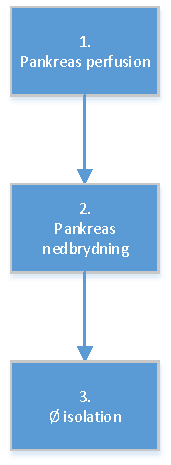
\includegraphics[width=0.2\textwidth]{billeder/sortering-crop.pdf}
	\caption{Faser i sorteringsprocessen}
	\label{fig:sortproces}
\end{figure}

I første fase, \textit{pankreas perfusion}, sprøjtes enzymet \textit{collagenase V} ind gennem galdegangene og derfra videre til  pankreas. Dette enzym starter en nedbrydning af vævet i pankreas. Herefter fjernes pankreas operativt. Enzymet collagenase har den egenskab, at det ikke nedbryder de langerhanske øer i samme grad som det omkringliggende eksokrine væv.

I anden fase, \textit{pankreas nedbrydning}, nedbrydes pankreas yderligere ved at inkubere pankreas ved 37° i 19 min. Ved denne temperatur er enzymet collagenase særligt aktivt og katalysere derfor nedbrydningen af pankreas. Herefter nedkøles vævet for at stoppe virkningen af collagenase.

% sker derfor relativt hurtigt.  den bliver skåret i mindre dele og pankreas placeres i en inkubator ved 37,5 grader. Dette gøres for at accelerere nedbrydningen af pankreas. Når pankreas er nedbrudt nedkøles vævet for, at stoppe virkningen af collagenase. 

I den sidste fase, \textit{ø isolation}, vaskes og rystes øerne først af tre omgange med en vaskebuffer i form af en saltvandsopløsning \citep{hbbs}. Dette gøres for at løsrive øerne fra hinanden inden isolering. Herefter er øerne klar til at blive isoleret fra det eksokrine væv. Der findes en række forskellige metoder til dette, hvor den mest udbredte metode foregår ved manuel isolering af øerne fra en petriskål vha. et mikroskop. Der bruges allerede automatiserede isoleringsmetoder bygget på forskellige teknikker, herunder gradientbaseret centrifugering. Fælles for de anvendte teknikker til isolering af øerne er, at der er stor risiko for skade på øerne. 

Denne manuelle metode har yderligere ulemper, idet den både er besværlig og tidskrævende. Herudover kan der være stor variation i kvaliteten af isoleringen, da der kan være forskel på den enkelte operatørs håndtering af øerne. 

Derfor ønskes der en automatiseret metode til isolering af langerhanske øer, med minimal risiko for skader på øerne. En automatiseret metode vil have følgende fordele \cite{pptintro}: 

\begin{itemize}
\item Øget sorteringshastighed for højere udbytte
\item Reducere variation i de isolerede øer
\item Reducere omkostningerne
\item Sikre bedre dokumentation
\item Forbedret arbejdsmiljø
\end{itemize} 

En automatiseret løsning vil potentielt åbne op for nye muligheder indenfor anvendelse af langerhanske øer. Der forskes bl.a. i transplantation af langerhanske øer, som et led i behandling af type 1 diabetes. Resultaterne af et af disse forskningsprojekter har bl.a. vist at 44 \% af modtagerne af denne type behandling var insulinuafhængige 3 år efter transplantation \citep{islettransplantation}. Til forskning er langerhanske øer bl.a. anvendt til at undersøge hvordan aminosyrer er glukoseafhængige \citep{aminosyre}. I forskningsforsøget er der brugt 6-10 mus, hvilket cirka har taget 6-10 timer at håndplukke (jvf. Per B. Jeppesen). Det er forskningsprojekter som dette, hvor en automatiseret løsning vil være relevant, da det vil skabe en mulighed for en større testgruppe og frigive ressourcer til andre formål i forsøget.

\newpage
På Medicinsk Endokrinologisk Afdeling (MEA), Aarhus Universitetshospital, er der tidligere arbejdet hen imod en automatiseret løsning til isolering af langerhanske øer. Den automatiseret løsning vil primært bidrage til forskningen, der foretages på afdelingen. Tidligere blev der udviklet en prototype til automatiseret ø-isolation, der fungerede ved hjælp af kameradetektion. Ved detektion sugede en pipette den detekterede ø op fra en petriskål. Pipetten blev styret i X,Y og Z retning vha. en mekanisk robotarm. Se figur \ref{fig:Tidliger prototype} for en illustration af den gamle prototype. \footnote{Kilde: Søren Gregersen}

\begin{figure}[H]
	\centering
	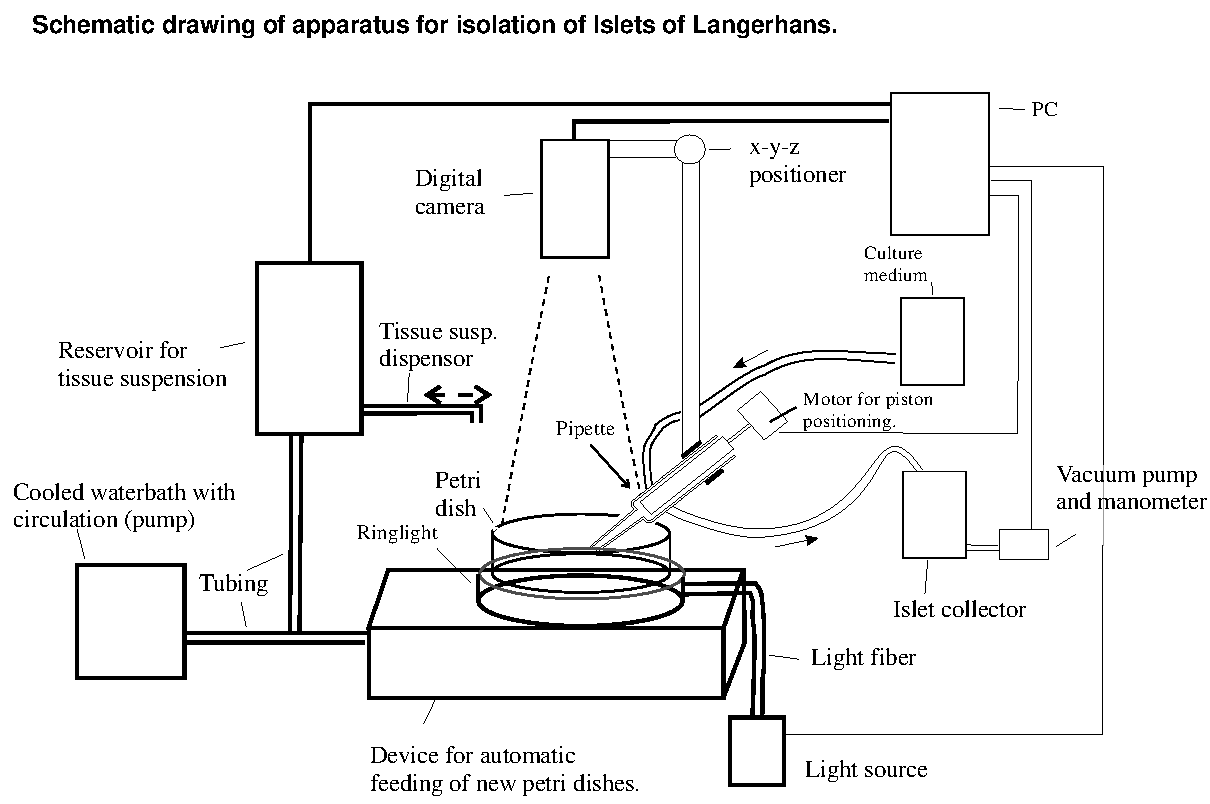
\includegraphics[width=1\textwidth]{billeder/hovedrapport/glprototype.pdf}
	\caption{Tidligere prototype}
	\label{fig:Tidliger prototype}
\end{figure}


 Prototypen var dog ikke præcis nok, primært pga. bevægelse i væsken, og projektet blev derfor stoppet.
 

%\textbf{Noter:}
%
%kilder om transplantation af øer
%
%
% 
% 
% find videnskabelige artikler der bekræfter at denne metode med at skyde langerhanske øer ind i sukkersyge mus/rotter virker og det er derfor dette projekt er mega relevant og pisse godt
% 
% derfor
% 
% - videnskabelig artikel over sorteringsprocessen
% 
% - videnskabelig artikel over at metoden virker, evt. hvorfor den ikke er mere brugt(sorteringsprocessen er for langsommelig)


\include{bilag/datablade}

%\chapter{Resultater}

\section{Det færdige system}
- Kamera

\section{Cost-benefit analyse}
Økonomisk

Andre ting?
%\chapter{Resultater}

\section{Det færdige system}
- Kamera

\section{Cost-benefit analyse}
Økonomisk

Andre ting?
%\chapter{Resultater}

\section{Det færdige system}
- Kamera

\section{Cost-benefit analyse}
Økonomisk

Andre ting?

%% Afrunding %%

%\section{Konklusion}
husk at problemformuleringenspunkter skal kunne afkrydses her nede


%%%% Kilder %%%%

\begingroup
	\raggedright
	\bibliography{bibtex/litteratur}							% Litteraturlisten inkluderes
\endgroup


%%%% Fixme-listen %%%%

\newpage														% Ny side til Fixme-listen
\listoffixmes													% Fixme-listen - fjernes til sidst i projektet med "%"


%%%% Appendiks %%%%

\appendix														% Appendiks/bilag start - giver chapter bogstaver i stedet for tal
\clearforchapter												% Sikrer at pagestylen aktiveres paa den rigtige side
\phantomsection													% Kunstigt afsnit, som hyperlinks kan 'holde fast i'
\pdfbookmark[0]{Appendiks}{appendiks}							% Tildeler en klikbar bookmark til den endelige PDF

%% Indstillinger for appendiks (deaktiveret med "%") %%

%\pagestyle{empty}												% Sidehoved/-fod for standardsider aendres til tom for appendiks
%\aliaspagestyle{chapter}{empty}								% Sidehoved/-fod for kapitelsider aendres til tom for appendiks
%\settocdepth{chapter}											% Kun kapitel-niveau vises i ToC
%\addtocontents{toc}{\protect\cftpagenumbersoff{chapter}}		% Sidetal for kapitler fjernes i ToC

%% Filer til appendiks %%
\chapter{Bilag}
\section{Datablade}
\subsection{INA114}
\label{bilag:INA114}
\subsection{L293D}
\label{bilag:L293D}

\subsection{L5-W55N-BVW}
\label{bilag:L5-W55N-BVW}

\subsection{161T031}
\label{bilag:161T031}

\section{Matlab kode}
Alt Matlab kode er vedlagt som .m filer i mappen ... 
\subsection{initArduino.m} \label{bilag:initArduino}
\subsection{cameraFeed.m} \label{bilag:cameraFeed}
\subsection{detectIslets.m}
\subsection{loadCell.m}
\subsection{Imagesimulator.m} \label{bilag:camsimulation}
\section{Arduino Testkode}
\subsection{Kode til enhedstest til vægtcelle.pdf} 
\label{bilag:TKloadcell}
\subsection{Kode til enhedstest til pumpe.pdf}
\label{bilag:TKpumpe}
\subsection{Kode til enhedstest til ventil.pdf}
\label{bilag:TKventil}


%%%% Bilag %%%%

%\phantomsection												% Kunstigt afsnit, som hyperlinks kan 'holde fast i'
%\addcontentsline{toc}{chapter}{Bilag A \ Navn} 				% Manuelle indgange i indholdsfortegnelsen (naar \includepdf bruges)

%\includepdf[pages={x-y}]{filnavn}								% Inkluder eksterne bilag med \includepdf[pages={x-y}]{filnavn}


\end{document}													% Slutter dokumentet - obligatorisk


